\newpage
\section{Textures}
To make 3D images realistic great detail is required. However assigning \textbf{different} materials to large number of \textbf{very small} triangles is \textbf{not feasible} due to memory requirements. The common approach uses \textbf{tables  } to assign different values to the parameters (color of the diffuse material,color of ambient light, color of specular term ecc..)of the shaders for the internal points of the surface. Most commonly such tables contain the \textbf{diffuse color} of the objects, acquired from an image. The considered tables ( or \textbf{images} )  are called \textbf{textures} (or maps).\\
Textures can be :
\begin{itemize}
\item 1D
\item 2D $\rightarrow$ in this course
\item 3D
\end{itemize}
Texture images that define the surface of an object are \textbf{planar} . However the objects in a scene often have \textbf{complex non-planar} topology.
\begin{figure}[H]
  \centering
  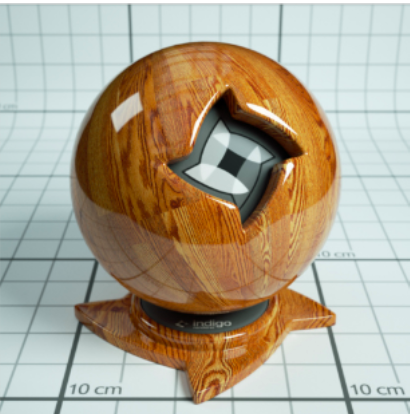
\includegraphics[width=.3\linewidth]{textures1}
\end{figure}
2D textures are applied to 3D objects using a \textbf{mapping relation} that associates each point on the surface with a point on the texture. The mapping creates a correspondence between pixels of the textures (\textbf{texels}) and points of the object.
\begin{figure}[H]
  \centering
  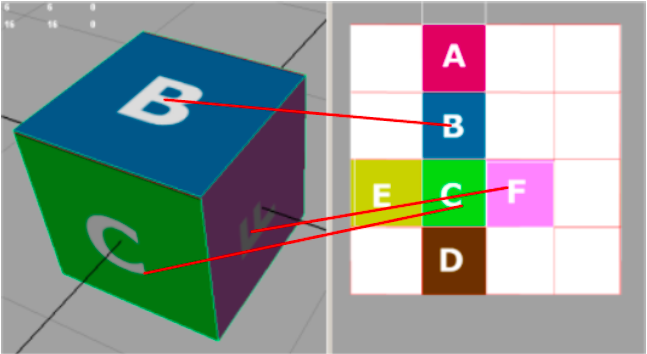
\includegraphics[width=.3\linewidth]{mapping}
\end{figure}
As seen in the figure above this often leads to unused areas of the texture ( see white spaces).\\
In case of  \textbf{polygonal} objects the mapping create a correspondence between \textbf{triangles of the mesh} and \textbf{triangles over the texture}
\begin{figure}[H]
  \centering
  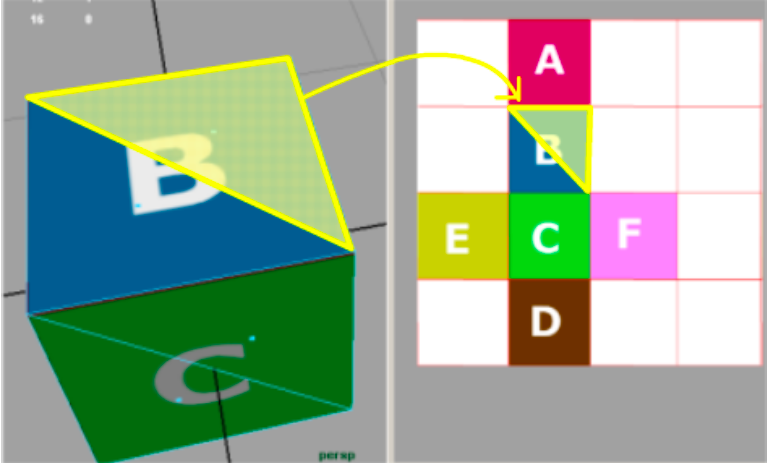
\includegraphics[width=.3\linewidth]{mapping2}
\end{figure}
Point of the 2D textures are addressed using \textbf{UV Coordinates } ( Cartesian coordinates with axes u and v)
\begin{figure}[H]
  \centering
  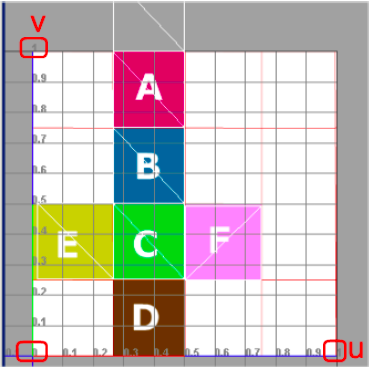
\includegraphics[width=.3\linewidth]{uvcoor}
\end{figure}
The coordinates range between 0 and 1 which implies that all texture images, regardless of their aspect ratio are \textbf{stretched} to fit into a square.
UV coordinates are \textbf{only} assigned to the \textbf{vertexes} of the triangles.
\\Vertex now have 8 components : 
\begin{itemize}
\item positional values $x,y,z$ to support projection
\item normal values $n_x,n_y,n_z$ to support smooth shading
\item UV Coordinates $u,v$ to support textures
\end{itemize}
\begin{figure}[H]
  \centering
  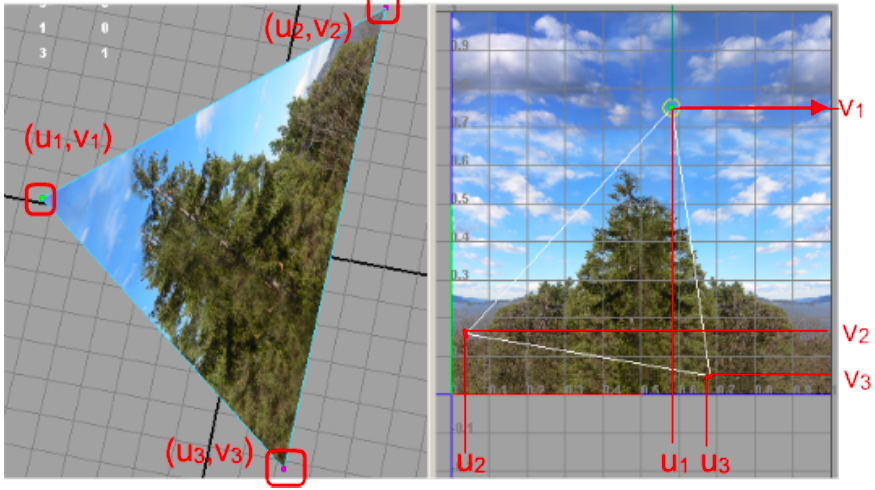
\includegraphics[width=.5\linewidth]{uvcoor1}
\end{figure}
Internal points are then interpolated
\begin{figure}[H]
  \centering
  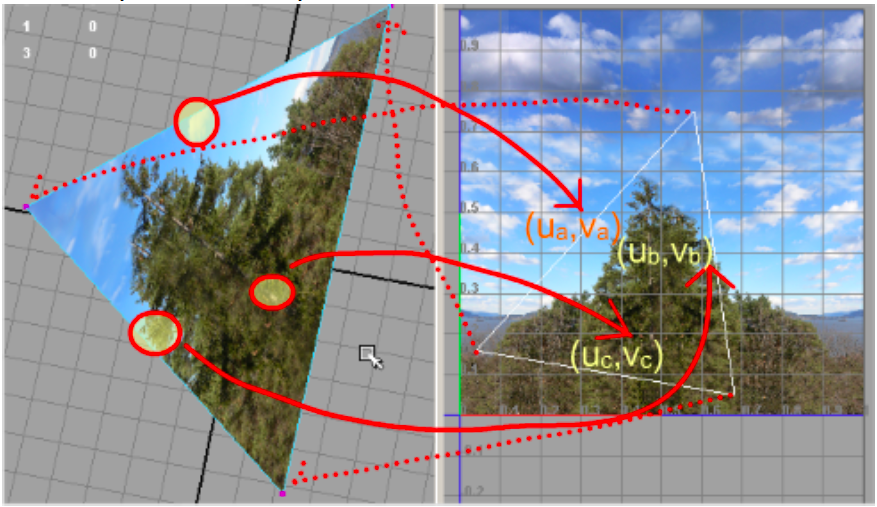
\includegraphics[width=.5\linewidth]{uvcoor2}
\end{figure}
The more the shape  of the triangles defined in the objects and the triangles of the texture are similar the \textbf{less distorted} will be the applied texture. This matching process is very long and tedious.
\begin{figure}[H]
  \centering
  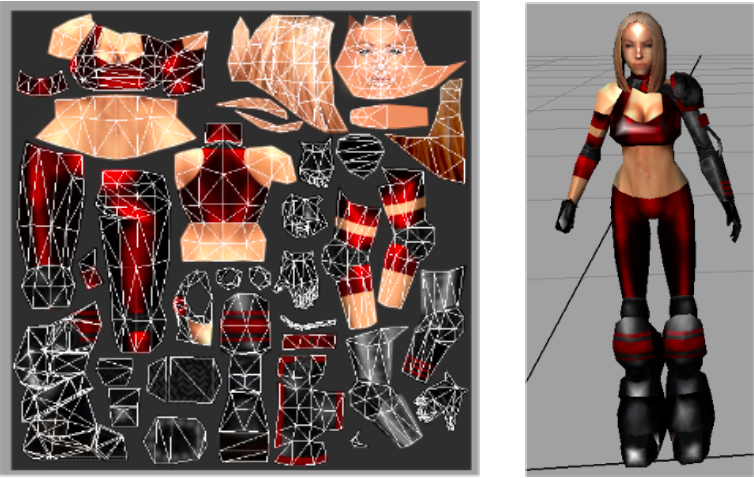
\includegraphics[width=.4\linewidth]{uvcoor3}
\end{figure}
As seen above mapping is not a \textbf{bijection} : the same part  of the texture can be shared by several triangles of the 3D object. This feature can be exploited to reduce memory usage.
\newpage
\subsubsection{Perspective interpolation}
Conventional interpolation often leads to \textbf{wobbling} images if \textbf{perspective} is used.
\begin{figure}[H]
  \centering
  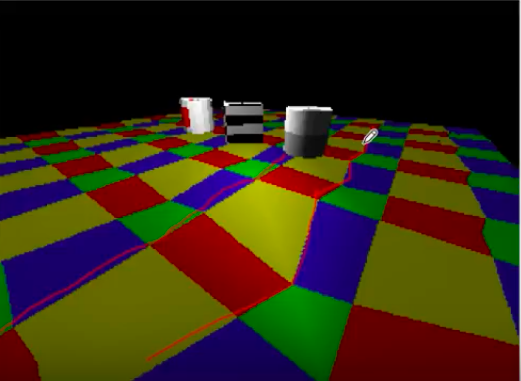
\includegraphics[width=.4\linewidth]{wobbling}
\end{figure}
This problem is not only restricted to the textures parameters but also affects parameters like the normal vectors or colors. However for those other parameters the perspective effect is \textbf{less perceivable} and can be easily corrected with linear approximations.\\
An example is provided to explain why perspective interpolation is a problem for textures. Two points in a 3D space are given with \textbf{u-coordinate} and \textbf{z-coordinate} (distance from projection plane):
\begin{itemize}
\item \textbf{P1} has $u_1 = \frac{1}{2}$ , $z_1 = 0.3$
\item \textbf{P2} has $u_2 = 1$ , $z_1 = 0.1$ 
\end{itemize}
The two points are projected on the projection plane at coordinates
$$ y_{S1}= 20$$
$$ y_{S2}= 26$$
\begin{figure}[H]
  \centering
  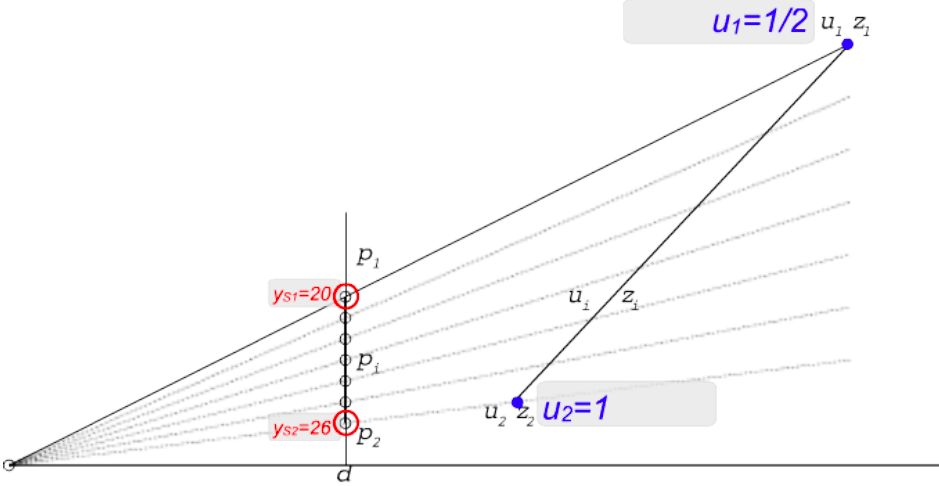
\includegraphics[width=.5\linewidth]{perspinter}
\end{figure}
So the pixels at coordinate $ y_{S1}= 20$ and $ y_{S2}= 26$ will have \textbf{u-coordinate} ,respectively, $u_1 = \frac{1}{2}$ and $u_2 = 1$. In a 3D space the u-coordinates vary \textbf{linearly}. Since there are 5 points between the two y coordinates , spacing the u-coordinates linearly results in the following:
\begin{figure}[H]
  \centering
  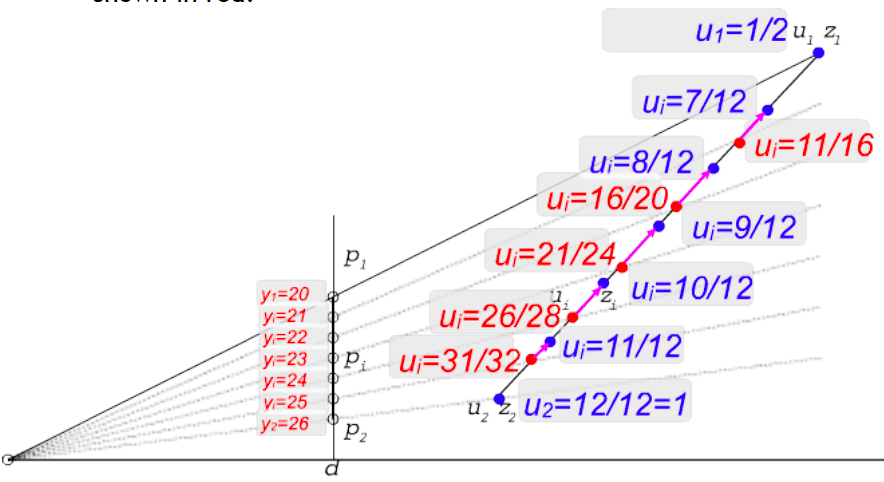
\includegraphics[width=.5\linewidth]{perspinter2}
\end{figure}
In blue we can see the equally-spaced points that match the linear case. Unfortunately the actual values ( seen in red ) are found in a different manner because the inverse projection of 2D coordinates in 3D space is \textbf{non-linear}.
To solve this issue \textbf{perspective correct interpolation} is used.\\
Consider parameter u which assumes values $u_1$ at $z_1$ and $u_2$ at $z_2$. The aim is to find the perspective correct value $u(y_S)$ of the parameter $u$ in 3D space, corresponding to a pixel $y_S$ on screen .
\begin{figure}[H]
  \centering
  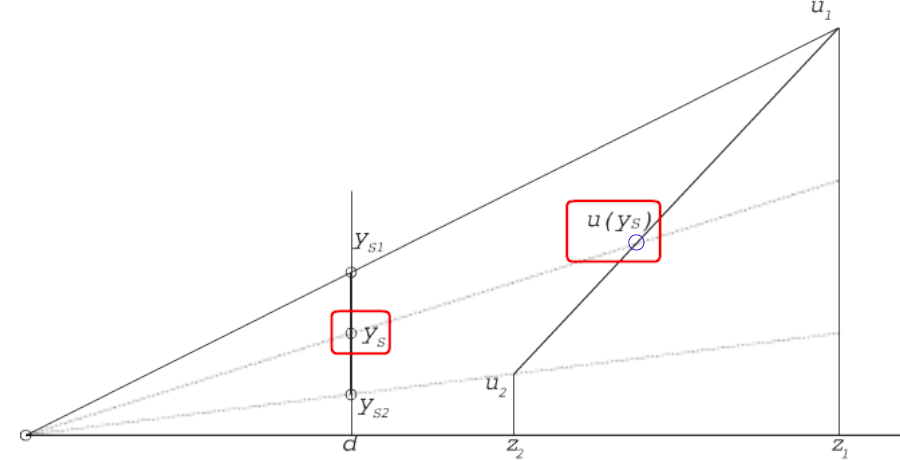
\includegraphics[width=.5\linewidth]{perspinter3}
\end{figure}
Recalling that $$y_{S1} = \frac{y_1}{\frac{z_1}{d}}$$ $$y_{S2} = \frac{y_2}{\frac{z_1}{d}}$$ $$ ... $$ $$y_{Si} = \frac{y_i}{\frac{z_i}{d}}$$
Since $u$ is \textbf{linear in 3D space} it can be expressed as a linear combination of its value at the two extremes $$ u(y_S) = \beta u_1 + (1-\beta)u_2$$
$$ x= \beta x_1 + (1-\beta)x_2$$
$$ y = \beta y_1 + (1-\beta)y_2$$
$$ z = \beta z_1 + (1-\beta)z_2$$
Also the pixel position on screen is \textbf{linear combination}:
$$ y_S = y_{S1}\alpha + y_{S2} (1-\alpha)$$
The goal is to find a relationship $ \alpha \rightarrow \beta$ :  
$$ u(y_{S1}\alpha + y_{S2}(1-\alpha))= u_1 \cdot \beta(\alpha)+ u_2 \cdot (1-\beta(\alpha)) $$
\begin{enumerate}
\item $ y_S = y_{S1}\alpha + y_{S2} (1-\alpha) \rightarrow \alpha = \frac{y_S - y_{S2}}{y_{S1} - y_{S2} }$
\item Since $y_{Si} = \frac{y_i}{\frac{z_i}{d}} \rightarrow y_S = \alpha \left(\frac{y_1}{\frac{z_1}{d}} \right) + (1-\alpha) \left(\frac{y_2}{\frac{z_2}{d}}\right)$
\item Since $y_S$ can be also found by interpolating separately y and z coordinate using factor $\beta$ and then \textbf{projection} the result : $y_S = \frac{\beta y_1 + (1-\beta) y_2}{\frac{\beta z_1 + (1-\beta)z_2}{d}}$
\item  $\alpha \left(\frac{y_1}{\frac{z_1}{d}} \right) + (1-\alpha) \left(\frac{y_2}{\frac{z_2}{d}}\right) =\frac{\beta y_1 + (1-\beta) y_2}{\frac{\beta z_1 + (1-\beta)z_2}{d}} $
\item After some simplifications and computations : \[ \boxed{\beta = \frac{\frac{\alpha}{z_1}}{\frac{\alpha}{z_1}+ \frac{(1-\alpha)}{z_2}}} \]
\end{enumerate}
Since $u(\alpha) = u_1\beta(\alpha)+ u_2(1-\beta(\alpha))$ : 
\[
\boxed{u(\alpha)= \frac{\alpha \frac{u_1}{z_1}+(1-\alpha) \frac{u_2}{z_2}}{\frac{\alpha}{z_1}+\frac{(1-\alpha)}{z_2}}}
\]
Generally an internal point of a triangle on screen can be considered a linear combination of its three vertices where the coefficients sum up to 1 : 
$$ (x_s,y_s) = (x_1,y_1) \cdot \alpha_1 + (x_2,y_2)\cdot \alpha_2 + (x_3,y_3)\cdot \alpha_3$$ $$ \alpha_1 + \alpha_2 + \alpha_3 = 1$$ So the value $u_S$ of $(x_S,y_S)$ is :
\[
\boxed{u_S=u(\alpha_1,\alpha_2,\alpha_3)= \frac{\alpha_1 \frac{u_1}{z_1}+\alpha_2 \frac{u_2}{z_2} + \alpha_3 \frac{u_3}{z_3}}{\frac{\alpha_1}{z_1}+\frac{\alpha_2}{z_2} + \frac{\alpha_3}{z_3}}}
\]
This process of correct interpolation should be done for all parameters considered \textbf{after the perspective projection}. As seen this method requires the distance of the point from the center of projection along the negative z-axis which corresponds to the \textbf{fourth component} of the \textbf{homogeneous coordinate vector changed of sign}
\begin{figure}[H]
  \centering
  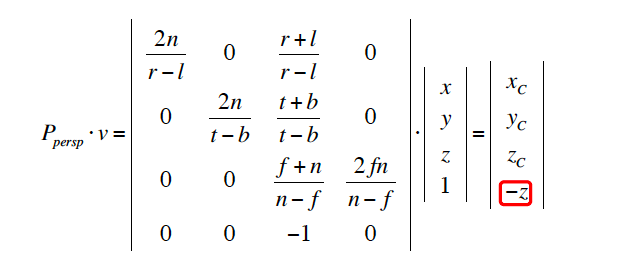
\includegraphics[width=.5\linewidth]{fourthcomp} 
\end{figure}